\subsection{RL-based operator selection} 
The performance of Variable Neighborhood Descent depends not only on the quality of the available neighborhood operators but also on the order in which they are explored. In the original GVNS and in the enhanced GVNS+ framework, neighborhoods are evaluated according to a predefined sequence composed of insertion, swap, relocation, exchange, and route-improvement operators. Although such a deterministic strategy provides stable performance, it assumes that the same neighborhood ordering remains appropriate throughout the entire optimization process.

In practice, the effectiveness of a neighborhood strongly depends on the current search context. Large structural moves may be beneficial immediately after diversification phases, whereas smaller operators often become more effective near local optima. Similarly, the most promising neighborhood may vary according to feasibility status, search stagnation, instance characteristics, and the recent evolution of solution quality. Consequently, a fixed neighborhood ordering may fail to exploit the search dynamics efficiently.

To address this limitation, neighborhood selection is formulated as a sequential decision-making problem solved through reinforcement learning. Instead of exploring neighborhoods according to a predefined order, the algorithm dynamically selects the operator that appears most promising given the current optimization state.

\subsubsection{MDP Formulation}
The adaptive operator-selection problem is modeled as a Markov Decision Process (MDP) embedded within the BVND intensification phase.

At each decision step, the learning agent observes a compact representation of the current optimization context and selects one neighborhood operator from the GVNS+ portfolio. The selected operator is applied to the current solution, producing a new search state and a reward that reflects the quality of the obtained improvement.

The state representation follows the unified search-state formulation introduced in Section~\ref{sec:baseline}. Rather than encoding complete routing solutions, which would be computationally prohibitive, the search process is described through a set of aggregated descriptors characterizing four complementary aspects of the optimization context:

\begin{itemize}
\item instance-level characteristics,
\item current solution quality and feasibility pressure,
\item search dynamics and stagnation indicators,
\item neighborhood effectiveness statistics.
\end{itemize}

This representation provides sufficient information for decision making while remaining computationally lightweight.

The action space corresponds directly to the eight neighborhood operators available in GVNS+:

\begin{equation}
A=\{N_1,N_2,\ldots,N_8\}.
\end{equation}

Each action represents the selection of one neighborhood operator for the next local-search step.

The reward is based on the improvement achieved in the augmented objective function. Let $F_t$ denote the objective value before applying the selected operator and $F_{t+1}$ the value obtained afterward. The normalized improvement is defined as

\begin{equation}
r_t=\frac{F_t-F_{t+1}}{1+F_t}.
\end{equation}

Additional reward shaping terms are introduced to encourage feasibility improvements and discourage ineffective neighborhood selections. Detailed reward definitions for each learning model are provided in Appendix~B.

Following the application of the selected operator, the optimization context is updated and becomes the next state observed by the agent. The learning process continues until the termination criterion of the outer GVNS+ search is reached.

\subsubsection{Integration within GVNS+}
Figure~\ref{fig:rl_gvns_architecture} illustrates the integration of reinforcement learning within the GVNS+ framework.

\begin{figure}[ht]
\centering
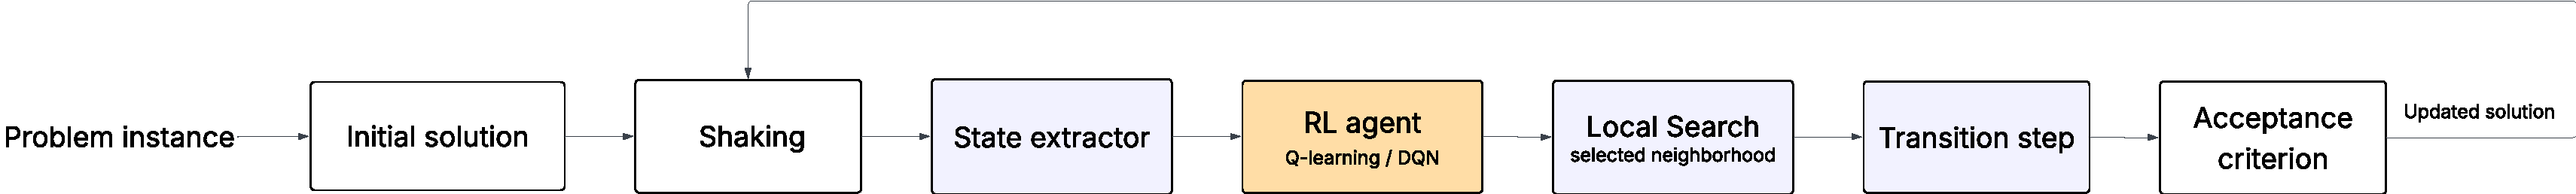
\includegraphics[width=\linewidth]
{../figures/rl_gvns_architecture.pdf}

\caption{RL-driven GVNS+ architecture}
\label{fig:rl_gvns_architecture}
\end{figure}

At each GVNS+ iteration, the shaking phase first generates a perturbed solution intended to escape the current local optimum. The search-state representation is then extracted and provided to the RL agent. Based on this information, the agent selects one neighborhood operator to be executed during the subsequent intensification step.

The selected neighborhood is applied through a single-neighborhood BVND iteration, generating a candidate solution. The environment then evaluates the resulting improvement, computes the reward, and updates the state representation. This transition is used by the learning algorithm to refine its decision policy. Finally, the candidate solution is processed by the GVNS+ acceptance mechanism before the search proceeds to the next iteration.

This integration preserves the overall structure of GVNS+ while replacing the static neighborhood-ordering mechanism with an adaptive decision process capable of reacting to the current optimization context.

\subsubsection{Tabular Q-Learning Agent}
The first adaptive operator-selection strategy is based on tabular Q-learning \cite{sutton2018reinforcement}. The objective is to learn the expected long-term utility of each neighborhood operator under different search conditions.

Because tabular reinforcement learning requires a finite state space, the continuous search descriptors are transformed into a compact abstract representation. The abstraction combines feasibility indicators, stagnation information, neighborhood-performance statistics, and instance-size categories. The resulting state space remains sufficiently small to enable efficient learning while preserving the main characteristics of the optimization context.

\begin{table}[ht]
\centering
\caption{State abstraction used by the Q-learning agent}
\label{tab:qlearning_state}

\begin{tabular}{lll}
\hline
Feature & Description & Levels\\
\hline
Feasibility status & Constraint violations & 3\\
Stagnation level & Search progress & 4\\
Neighborhood effectiveness & Recent performance & 4\\
Instance size bucket & Problem scale & 3\\
\hline
\end{tabular}

\end{table}

The agent maintains a Q-table storing an estimate of the expected cumulative reward associated with each state-action pair. After observing a transition $(s,a,r,s')$, the table is updated according to the classical Bellman update rule:

\begin{equation}
Q(s,a)\leftarrow Q(s,a)+
\alpha
\left[
r+\gamma \max_{a'}Q(s',a')
-Q(s,a)
\right].
\end{equation}

Action selection is performed using an Upper Confidence Bound (UCB) strategy, which balances exploration and exploitation by considering both the estimated value of an action and the number of times it has been previously selected. Compared with standard $\epsilon$-greedy exploration, UCB promotes a more structured exploration process and is particularly suitable for adaptive metaheuristics where neighborhood effectiveness evolves throughout the search.

\subsubsection{Deep Q-Network Agent}
Although tabular Q-learning provides an interpretable adaptive mechanism, its reliance on state discretization limits its ability to capture fine-grained variations in the optimization process. To overcome this limitation, a Deep Q-Network (DQN) \cite{mnih2015human} is also investigated.

Unlike tabular Q-learning, DQN approximates the action-value function through a neural network operating directly on the continuous search-state representation. This eliminates the need for manual state discretization and enables the model to learn more complex relationships between optimization states and neighborhood effectiveness.

The adopted network architecture is shown in Figure~\ref{fig:dqn_architecture}. The model consists of a multilayer perceptron with two hidden layers of 128 neurons each and ReLU activation functions. The output layer contains one neuron for each neighborhood operator and produces the estimated action values $Q(s,a)$.

\begin{figure}[ht]
\centering
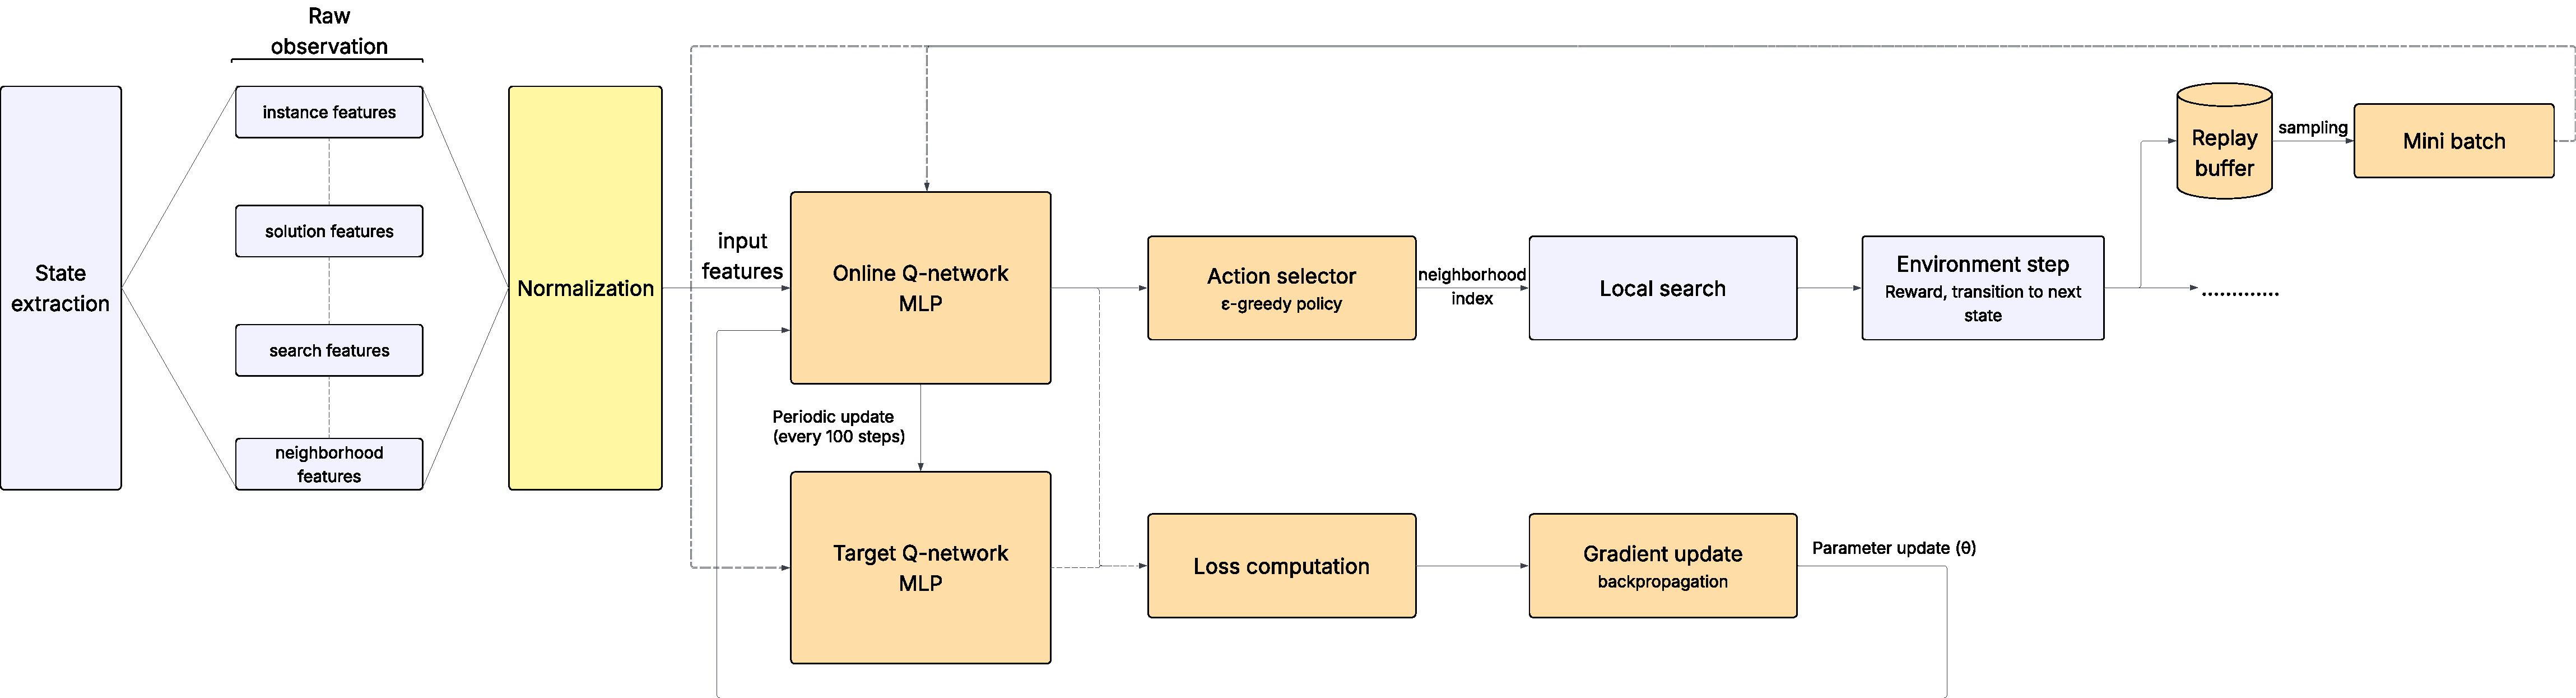
\includegraphics[width=\linewidth]
{../figures/dqn_architecture.pdf}

\caption{DQN architecture}
\label{fig:dqn_architecture}
\end{figure}

To improve learning stability across instances of different sizes, all state features are normalized online using running estimates of feature means and variances before being processed by the network. This prevents large-magnitude descriptors from dominating the learning process and improves generalization across heterogeneous routing instances.

Action selection follows an $\epsilon$-greedy exploration strategy. With probability $\epsilon$, a neighborhood is selected randomly; otherwise, the neighborhood associated with the largest predicted action value is chosen.

Experience replay and target-network mechanisms are employed during training to stabilize value estimation and reduce temporal correlations between consecutive observations. The network parameters are optimized by minimizing the temporal-difference error over mini-batches sampled from the replay buffer.